%%%%%%%%%%%%%%%%%%%%%%%%%%%%%%%%%%%%%%%%%%%%%%%%%%%%%%%%%%%%%%%%%%%%%%%%%%%%%%%%
\begin{figure}[ht!]
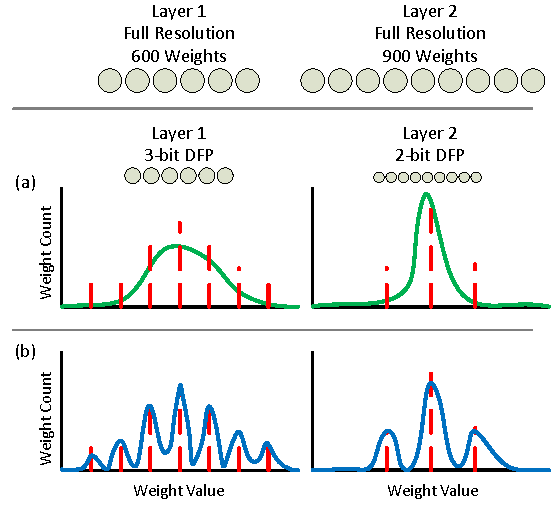
\includegraphics[width=\columnwidth]{img/intro2.pdf}
\caption{An example Network with two layers demonstrating (a) Layer-wise Precision Scaling (b) Retraining with Quantization-regularization. Starting with two layer network at first the bit-widths of both layers are adjusted by defining a lower precision format with the quantization levels marked as dotted lines in the histogram charts (a). To reduce the quantization error, retraining with additional regularization, decreasing the average distance of the weights to the quantization levels, is performed (b).}\label{fig:intro}
\end{figure}


\section{Motivational Case Study}
%The method proposed in this paper attacks the two biggest challenges for efficient DNN inference on resources restricted devices (\ref{sec:intro}). 
Figure \ref{fig:intro} explains with a simple example the two main parts of the paper. Assuming a two-layer neural network with two layers with 600 and 900 weights respectively, we want to achieve model compression by reducing the number of bits stored per weight and specific quantization of the weights to enhance the computational energy efficiency. 

First note, that layer 2 has a stronger impact on the size of the weight memory, as it contains more weights. Thus, it is beneficial in terms of memory footprint to reduce the bit-width of its weights more than those of layer 1. 
%While reducing the the bit-width equally for both layers decreases weight memory, layer 2 has a stronger impact on the size of the weight memory than layer 1.
However, quantization also negatively affects the accuracy of the algorithm, due to weight quantization errors. Therefore we apply Layer-wise Precision Scaling (Fig. \ref{fig:intro}a) to find the best trade-off between compression due to quantization and accuracy degradation.
While for the example in figure \ref{fig:intro} uniform 3-bit quantization leads to 4.5kbit weight memory, with Layer-wise Precision Scaling applied according to figure \ref{fig:intro}a only 3.6kbit weights need to be stored, allowing us to increase compression ratio by a factor 1.25.

To alleviate the accuracy degradation, performing trained quantization by applying additional regularization with the goal of reducing the weight quantization error results in an increase the accuracy. For state-of-the-art DNNs Layer-wise Precision Scaling shows even higher efficiency due to the higher variation of numbers of weights per layer (see table \ref{tab:allconv}).


%\textcolor{purple}{Try to come up something similar to the motivation paper		Idea: You can think of roughly comparing \# of multipliers in different n/ws (the ones u use in experiments) and u can assign some kind of delay to different multipliers (say 8-bit has delay of x, 16-bit multiplier has delay of y, and y>>x, so using 16-bit is much slower. In our case, we use 8+16 bit, so using this has some ax+by delay with accuracy xyz\%) something that gives people why this quantizations is needed }

